\section{Results}

\subsection{Weak Scaling}


\begin{figure}
\begin{subfigure}[b]{0.5\textwidth}
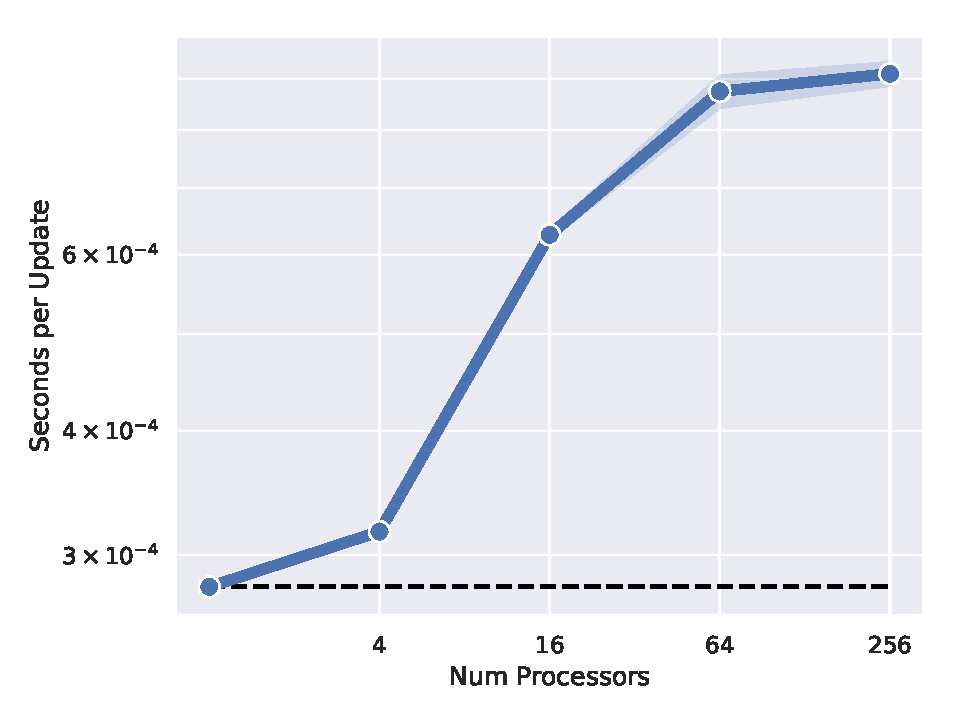
\includegraphics[width=\textwidth]{img/MPIWeak}
\caption{
MPI implementation
}
\label{fig:mpi_weak}
\end{subfigure}
\begin{subfigure}[b]{0.5\textwidth}
  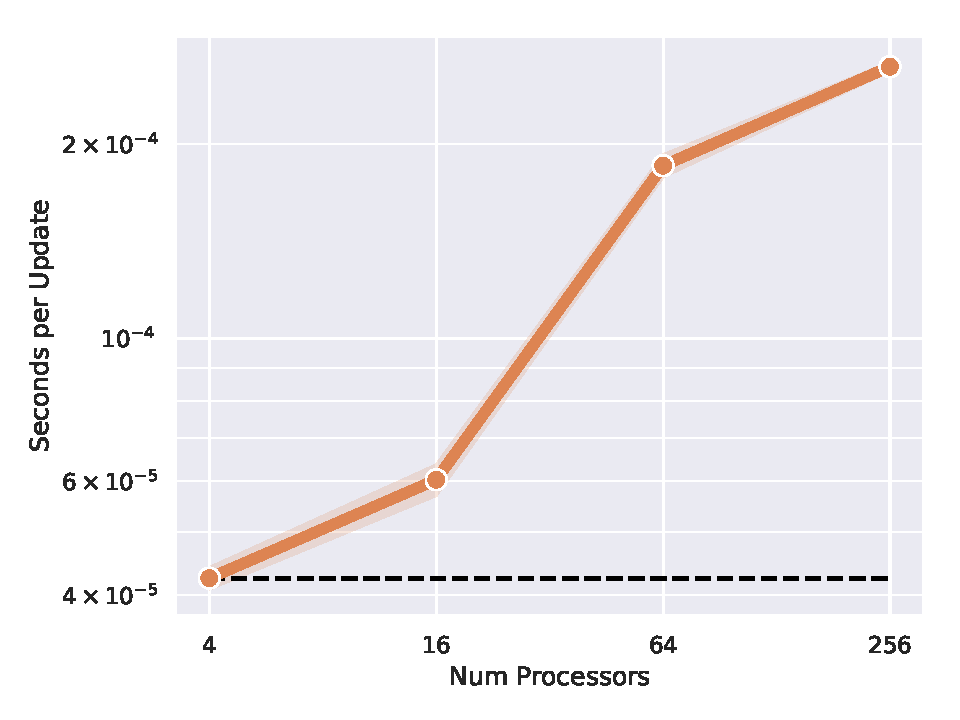
\includegraphics[width=\textwidth]{img/CharmWeak}
\caption{
Charm++ implementation
}
\label{fig:charm_weak}
\end{subfigure}
\caption{
Weak scaling analysis (time to solution versus parallelism with problem size proportional to parallelism) for MPI (\subref{fig:mpi_weak}) and Charm++ (\subref{fig:charm_weak}) implementations.
Dashed line indicates the ideal scaling relationship.
Shaded area represents standard deviation of five replications for each observation.
A problem size of 262,144 grid tiles per CPU was used for the MPI implementation and 1 grid tile per CPU was used for the Charm++ implementation.
}
\label{fig:weak}
\end{figure}


Figure \ref{fig:weak} shows the relationship between time-to-solution and parallelism with problem size growing proportionally to parallelism for both the MPI and Charm++ implementations.
Ideally, time-to-solution would remain unchanged as more work and more processors are added.
However, both implementations experience a large performance hit scaling through the range of about 4 to 64 processors.
As discussed in \label{sec:compute}, the HPCC allocated a compute environment with about 12 processors per node.
Thus, this large performance hit to both implementations is probably due to greater communication costs for communication between nodes.
Encouragingly, though, both implementations (but especially MPI) see a less severe reduction in performance scaling from 64 to 256 nodes, suggesting that scaling up further to even more nodes could be accomplished efficiently.

\subsection{Strong Scaling}


\begin{figure}
\begin{subfigure}[b]{0.5\textwidth}
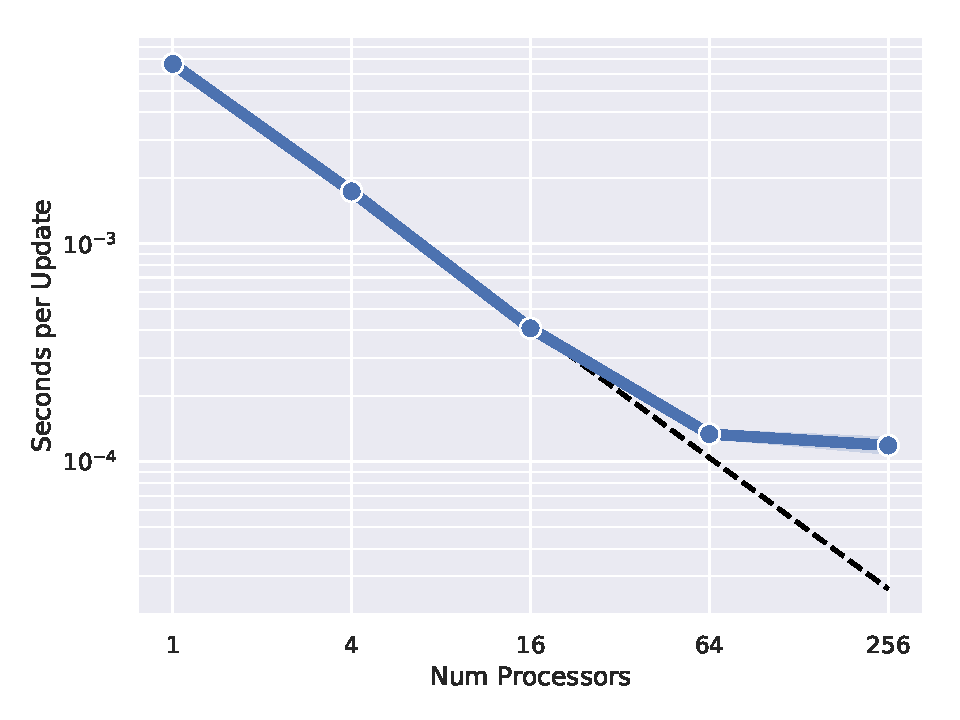
\includegraphics[width=\textwidth]{img/MPIStrong}
\caption{
MPI implementation
}
\label{fig:mpi_weak}
\end{subfigure}
\begin{subfigure}[b]{0.5\textwidth}
  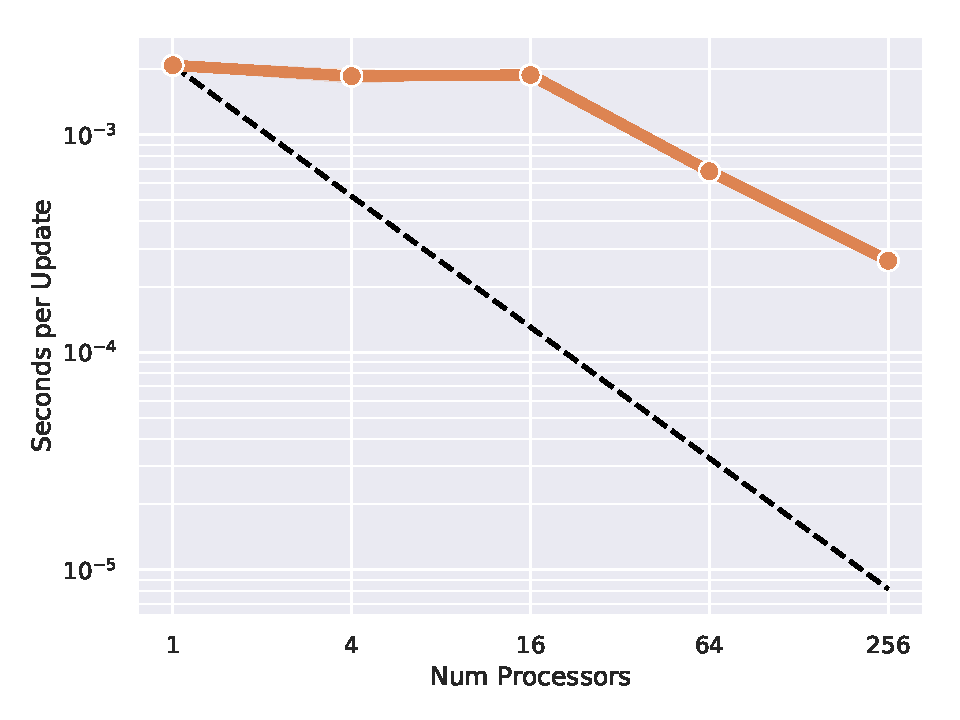
\includegraphics[width=\textwidth]{img/CharmStrong}
\caption{
Charm++ implementation
}
\label{fig:charm_weak}
\end{subfigure}
\caption{
Strong scaling analysis (time to solution versus parallelism for a fixed problem size) for MPI (\subref{fig:mpi_weak}) and Charm++ (\subref{fig:charm_weak}) implementations.
Dashed line indicates the ideal scaling relationship.
Shaded area represents standard deviation of five replications for each observation.
Fixed problem size was a $2048\times2048$ grid for the MPI implementation and a $16\times16$ grid for the Charm++ implementation.
}
\label{fig:strong}
\end{figure}


Figure \ref{fig:strong} shows the relationship between time-to-solution and parallelism with a fixed problem size for both the MPI and Charm++ implementations.

At an overall grid size of $2048 \times 2048$ MPI scales near-ideally up to 64 processors before speedup levels off.
At 256 processors, sub-grid size has decreased to $256\times256$.
The performance saturation at 64 processors is perhaps due to a breakdown of latency hiding: at that smaller sub-grid size there isn't enough work for each rank to do while waiting for communications to complete.

Our Charm++ strong-scaling study employed a grid size of $16 \times 16$ (256 tiles total).
Compared to the single-processor time-to-solution, Charm++ exhibits no increase in performance as the first 16 processors are added.
Then, as more processors are added time-to-solution begins to decline at a near-ideal rate.
At low processor counts, many Chare objects share the same CPU.
The lack of speedup at low processor counts might be due to Charm++ overhead involved with to schedule and un-scheduling many Chares on the same CPU.


\subsection{Verification}


\begin{figure}
\begin{subfigure}[b]{0.33\textwidth}
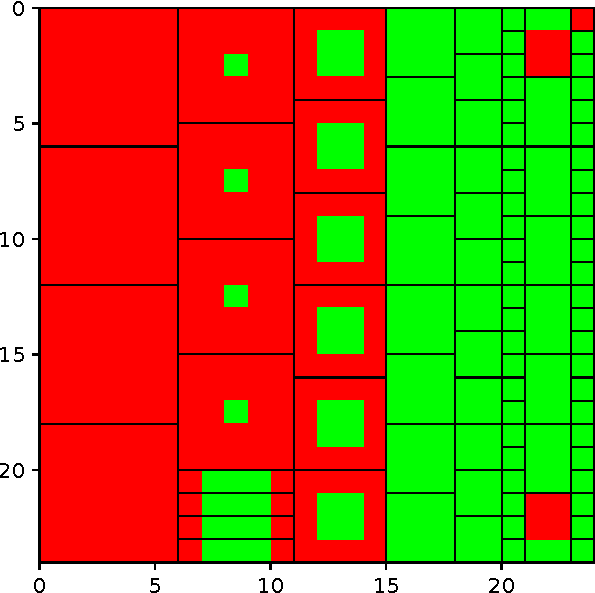
\includegraphics[width=\textwidth]{img/Charm-correctness}
\caption{
Charm++
}
\label{fig:charm_correctness}
\end{subfigure}%
\begin{subfigure}[b]{0.33\textwidth}
  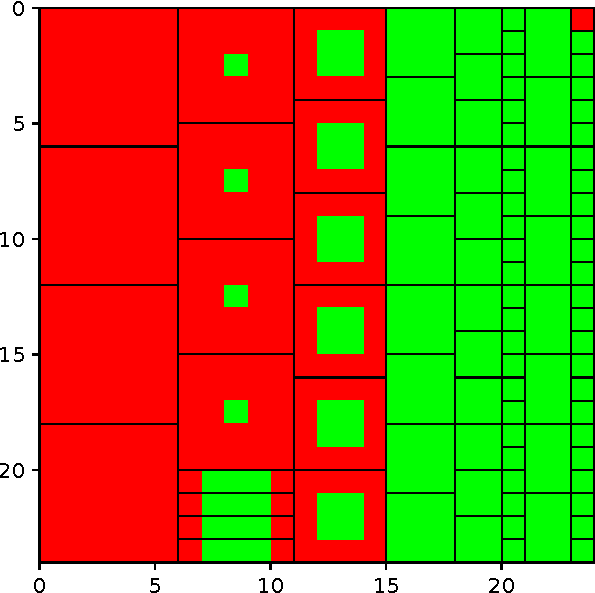
\includegraphics[width=\textwidth]{img/MPI-n1-correctness}
\caption{
MPI $n=1$
}
\label{fig:mpi_n1_correctness}
\end{subfigure}%
\begin{subfigure}[b]{0.33\textwidth}
  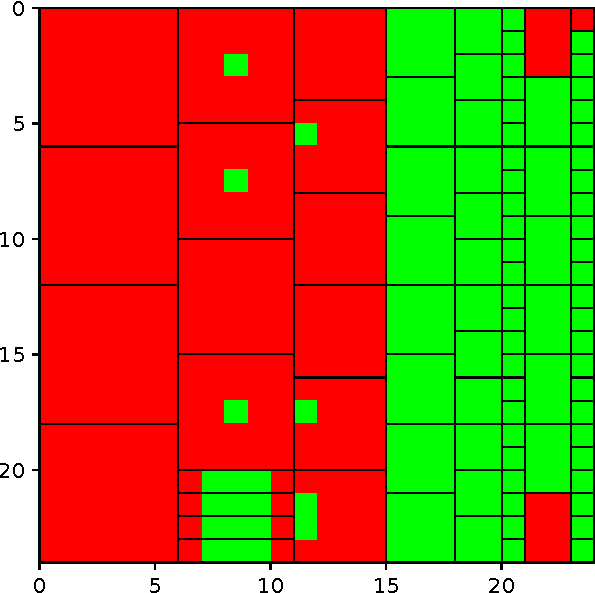
\includegraphics[width=\textwidth]{img/MPI-n4-correctness}
\caption{
MPI $n=4$
}
\label{fig:mpi_n4_correctness}
\end{subfigure}
\caption{
Final resource accumulations as verification of implementation correctness for Charm++ implementation (\subref{fig:charm_correctness}), MPI with $n=1$ (\subref{fig:mpi_n1_correctness}), and MPI with $n=4$ (\subref{fig:mpi_n4_correctness}).
Black lines indicate divisions between same-channel groups.
Red coloring indicates negative resource accumulation at a tile and green coloring indicates positive resource accumulation at a tile.
Note that the single upper-right hand tile is part of a contiguous same-channel group with the large upper-left same-channel group via toroidal wraparound and that the top and bottom $3 \times 2$ same-channel groups in columns 22 and 23 are a contiguous same-channel group via toroidal wraparound.
}
\label{fig:correctness}
\end{figure}


As with other endeavors in the field of Artificial Life \cite{bedau2000open}, our goal is to design and study an abstract system that experiences a phenomenon of interest rather than to directly model a specific (biological) system.
Because our the aim is ultimately generative instead of strictly emulative, our criteria for correctness isn't necessarily as strictly defined as that for other scientific software.

Although ideally avoided for reproducibility's sake, our objective is not incompatible with nondeterminism introduced by race conditions.
(In fact, demonstrating robustness to asynchrony and hardware hiccups/failure is perhaps useful for arguing that our approach is compatible with extreme computational scaling \cite{ackley2016indefinite}.)
At a fundamental level, our asynchronous Charm++ implementation is sensitive to hardware stochasticity (e.g., what order Charm++ messages are received and queued in).

Here are our criteria for correctness:
\begin{enumerate}
\item medium-sized same-channel groups accumulate resource at a greater rate than small and too-large same-channel groups, and
\item for the MPI implementation, our simulation yields exactly the same results on any number of processors.
\end{enumerate}

I verified the implementations by loading a manually-designed $24 \times 24$ channel layout and then inspecting resource accumulations at the end of a 150 second run.
The channel layout was designed with a general left-to-right gradient of same-channel group size, with a few same-channel groups wrapped around the toroidal edges.
Figure \ref{fig:correctness} shows resource accumulation results mapped over outlines of same-channel groups for the Charm++ implementation, for the MPI implementation with $n=1$, and for the MPI implementation with $n=4$.
See the figure caption for details on same-channel groups wrapped around the toroidal edges.

For these runs, a resource wave size of three units was used.
That means that any tile that is more than three grid steps away from another tile in its same-channel signaling group should experience negative resource accumulation.
The Charm++ implementation appears entirely correct: much-too-large cell groups exhibit completely negative resource accumulation, slightly-too-large cell groups exhibit negative resource accumulation at the periphery, and medium/small cell groups exhibit positive resource accumulation.
The MPI implementations are not entirely correct.
In the $n=1$ case, we don't have negative resource accumulation in the too-large top-to-bottom-wrapped same-channel group.
In the $n=4$ case, we have several sites at the interior of slightly-too-large cell groups where negative resource accumulation occurs where we would have expected positive resource accumulation and vice-versa.

The MPI implementation needs more debugging for correctness before it would be ready for research use.
However, the implementation suffices for meaningful performance profiling, which is the primary objective of the project at this stage.
